%%%%%%%%%%%%%%%%%%%%%%%%%%%%%%%%%%%%%%%%%%%%%%%%%%%%%%%%%%%%%%%%%%%%%%
% Lớp 11 | Giới hạn. Hàm số liên tục | Giới hạn của dãy số
% Dạng 1D3?1-6: Toán thực tế áp dụng giới hạn của dãy số
% Số câu: 22  (sinh tự động bởi tach_cau.py; từ nay thầy sửa trực tiếp file này)
%%%%%%%%%%%%%%%%%%%%%%%%%%%%%%%%%%%%%%%%%%%%%%%%%%%%%%%%%%%%%%%%%%%%%%

%%%%%%%%%%%%%%%% TRẢ LỜI NGẮN %%%%%%%%%%%%%%%%

% nguồn: Ok_TraLoiNgan_Lop11_Lan1
\begin{ex}%[1D3V1-6]%[ma:408235be]
	Người ta xếp các hình vuông kề với nhau như trong hình dưới đây, mỗi hình vuông có độ dài cạnh bằng nửa độ dài cạnh của hình vuông trước nó. Nếu hình vuông đầu tiên có cạnh dài $10$ cm thì trên tia $Ax$ cần có một đoạn thẳng dài bao nhiêu xentimet để có thể xếp được tất cả các hình vuông đó? 
	\begin{center}
		\begin{tikzpicture}
				\path 
					 (-1,0) coordinate (M)
					(0,0) coordinate (A) node at  (0,-0.4) {$A$}
					(0,4) coordinate  (B)
					(4,4)  coordinate (C)
					(4,0) coordinate  (D)
					(4,2) coordinate  (E)
					 (6,2) coordinate (F)
					(6,0)  coordinate (G)
					(6,1) coordinate (H) 
					 (7,1) coordinate (I)
					(7,0)  coordinate (J)
					(9,0)  coordinate (N) node at (9,-0.4) {$x$};
				 \draw
					 (A)--(B)--(C)--(D)--cycle
					 (E)--(F)--(G)
					(H)--(I)--(J); 
				 \draw [->] (A)--(N);
			\end{tikzpicture}
	\end{center}
	\shortans{20} 
	 \loigiai{Tổng các cạnh nằm trên tia $Ax$ của các hình vuông đó là
		\[10+5+\dfrac{5}{2}+\dfrac{5}{2^2}+\ldots=\dfrac{10}{1-\dfrac{1}{2}}=20 \text{  cm}.\]
	} 
\end{ex}

% nguồn: Ok_TraLoiNgan_Lop11_Lan1
\begin{ex}%[1D3V1-6]%[ma:99d9c270]
	Từ độ cao $300$ m, người ta thả một quả bóng cao su xuống đất. Giả sử cứ sau mỗi lần chạm đất, quả bóng nảy lên một độ cao bằng $\dfrac{1}{4}$ độ cao mà quả bóng đạt được trước đó. Gọi $h_n$ là độ cao quả bóng đạt được ở lần nảy thứ $n$. Gọi $S_n$ là tổng độ dài quãng đường  đi được của quả bóng từ lúc bắt đầu thả quả bóng đến khi quả bóng chạm đất lần thứ $n$. Tính $S_n$, nếu quá trình này cứ tiếp tục diễn ra mãi thì tổng quãng đường quả bóng di chuyển được là bao nhiêu?
	\shortans{400} 
	\loigiai{ 
		Ta thấy tổng $S_n$ là tổng của cấp số nhân lùi  vô hạn có $u_1=300$, công bội $q=\dfrac{1}{4}$.\\
		Ta  có $S_n=300+300\cdot\dfrac{1}{4}+300\cdot\left(\dfrac{1}{4}\right)^2+\ldots+300\cdot\left(\dfrac{1}{4}\right)^n+\ldots=300\cdot\dfrac{1}{1-\frac{1}{4}}=400$ m.
	} 
\end{ex}

% nguồn: Ok_TraLoiNgan_Lop11_Lan1
\begin{ex}%[1D3V1-6]%[ma:0481b652]
	Một bệnh nhân có vấn đề về thận, hàng ngày phải uống một viên thuốc $980$ mg. Từ ngày đầu đến ngày  thứ $10$, trước mỗi lần uống, hàm lượng thuốc cũ trong cơ thể vẫn còn $5 \%$. Tuy nhiên từ ngày thứ $11$ trở đi vì tình trạng thận được cải thiện nên trước mỗi lần uống thuốc, hàm lượng thuốc cũ trong cơ thể còn $2 \%$. Hãy uớc tính lượng thuốc trong cơ thể nếu bệnh nhân sử dụng thuốc trong một thởi gian dài.
	 \shortans{100}
	\loigiai{ 
		Gọi $u_n$ là lượng  thuốc trong cơ thể bệnh nhân sau khi uống ngày thứ $n$, ($n\ge 10$).\\
		Theo giả thiết  ta có
		$$u_{n+1}=98+2\% \cdot u_n, \forall  n \ge 10.\qquad(*)$$
		 Trừ hai vế của (*) với $100$ ta được
		$$(u_{n+1}-100)=2\%\cdot(u_n-100), \forall n \ge 10.$$ 
		Đặt dãy $(v_n)$ bởi $v_n=u_n-100, n\ge  10$. Khi đó dãy $\left( v_n\right)_{n\ge 10}$ là dãy cấp số nhân với công bội $q=2\%$ và số hạng thứ $10$ là $v_{10}=u_{10}-100$.\\
		Do đó 
		$$v_n=v_{10}\cdot  q^{n-10}=(u_{10}-100)\cdot 0{,}02^{n-10}, \forall n \ge 10.$$
		 Vì $0<0{,}02<1$ nên $\lim 0{,}02^{n-10} =0$.\\ Do đó
		$$\lim v_n =0 \Rightarrow \lim  u_n=100.$$
		Do đó nếu sử dụng lượng thuốc trong một thời gian dài, lượng thuốc trong cơ thể nếu  bệnh nhân duy trì khoảng $100$ mg.
	} 
\end{ex}

% nguồn: Ok_TraLoiNgan_Lop11_Lan2
\begin{ex}%[1D3V1-6]%[ma:8ee81956]
	Từ tờ giấy, cắt một hình tròn bán kính $R=2$ (cm). Tiếp theo, cắt hai hình tròn bán kính $\dfrac{R}{2}$ chồng lên hình tròn đầu tiên. Tiếp theo, cắt bốn hình tròn bán kính $\dfrac{R}{4}$  rồi chồng lên các hình trước. Cứ thế tiếp tục mãi như hình vẽ bên dưới. Tính tổng diện tích của các hình tròn (làm tròn kết quả đến hàng phần chục).
	\begin{center}
		\begin{tikzpicture}[declare function={r=3;}]
				\path 
					(0,0) coordinate  (O)
					(0:r) coordinate (A) 
					(180:r) coordinate (B) 
					($(A)!.5!(O)$) coordinate  (M)
					($(B)!.5!(O)$) coordinate  (N)
					($(B)!.5!(N)$) coordinate (I) 
					($(N)!.5!(O)$) coordinate (J) 
					($(O)!.5!(M)$)  coordinate (K)
					($(M)!.5!(A)$) coordinate  (H)
					($(B)!.5!(I)$)  coordinate (Q);
				 \draw (A) arc (0:360:r)
					(A) arc (0:360:r/2) 
					(O)  arc (0:360:r/2)
					(A) arc (0:360:r/4) 
					(A) arc (0:360:r/4) 
					(M) arc  (0:360:r/4)
					(O) arc (0:360:r/4) 
					(N) arc (0:360:r/4) 
					 (A) arc (0:360:r/8)
					(H)  arc (0:360:r/8)
					(M) arc  (0:360:r/8)
					 (K) arc (0:360:r/8)
					(O)  arc (0:360:r/8)
					(J) arc  (0:360:r/8)
					(N) arc  (0:360:r/8)
					(I) arc  (0:360:r/8);
				 \draw (A)--(B);
			\end{tikzpicture}
	\end{center}
	\shortans{25,1} 
	 \loigiai{
		Gọi $u_1$ là diện tích của hình tròn thứ  nhất, ta có $u_1=\pi R^2$.\\
		Gọi $u_2$ là tổng diện tích của $2^1$ hình tròn  cắt lần thứ hai, ta có $$u_2=2\pi \cdot\left(\dfrac{R}{2}\right)^2=\pi R^2\cdot \dfrac{1}{2}\, \left(\text{cm}^2\right).$$
		Gọi $u_3$ là tổng diện tích của $2^2$ hình  tròn cắt lần thứ ba, ta có $$u_3=4\pi \cdot\left(\dfrac{R}{4}\right)^2=\pi R^2\cdot \dfrac{1}{2^2}\, \left(\text{cm}^2\right).$$
		Gọi $u_n$ là tổng diện tích của $2^{n-1}$ hình tròn cắt lần thứ $n$, ta có $$u_n=2^{n-1}  \pi \cdot\left(\dfrac{R}{2^{n-1}}\right)^2=\pi R^2\cdot \dfrac{1}{2^{n-1}}\, \left(\text{cm}^2\right).$$
		Dãy $u_1$, $u_2$,  $u_3$, $\ldots$, $u_n$, $\ldots$ là cấp số nhân lùi vô hạn có số hạng đầu $u_1=\pi R^2$ và công bội $q=\dfrac{1}{2}$.\\
		Vậy tổng  diện tích của các hình tròn là
		\begin{eqnarray*}
			S&=&\pi  R^2+\pi R^2 \cdot \dfrac{1}{2}+\pi R^2 \cdot \dfrac{1}{2^2}+\ldots\\
			&=&\dfrac{\pi R^2}{1-\dfrac{1}{2}}\\ 
			 &=&2 \pi R^2\\
			 &=&2 \pi \cdot 2^2 \approx 25{,}1\, \left(\text{cm}^2\right).
		\end{eqnarray*}
	} 
\end{ex}

% nguồn: Ok_TraLoiNgan_Lop11_Lan2
\begin{ex}%[1D3V1-6]%[ma:97a88ac0]
	 \immini{
	Cho hình vuông cạnh $1$. Chia hình vuông đó thành bốn hình vuông nhỏ bằng nhau, sau đó tô màu hình vuông nhỏ góc dưới bên trái. Lặp lại các thao tác này với hình vuông nhỏ góc trên bên phải. Giả sử quá trình trên tiếp diễn vô hạn lần. Gọi $u_1, u_2, \ldots, u_n, \ldots$ lần  lượt là chu vi của các hình vuông được tô màu. Tính tổng chu vi của tất cả các hình vuông được tô màu.
	 }
	 {
	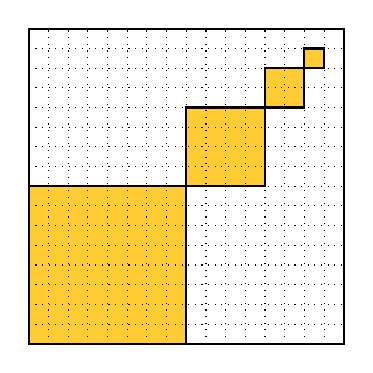
\begin{tikzpicture}
			\definecolor{myyellow}{rgb}{1,0.8,0.2} 
			\def\a{4} 
			\draw[thick]  (0,0) rectangle (\a,\a);
			 \foreach \i in {1,2,3,4}{
				\pgfmathsetmacro{\prev}{1 -  1/2^(\i-1)}
				 \pgfmathsetmacro{\curr}{1 - 1/2^\i}
				\pgfmathsetmacro{\size}{\a  * (1/2^\i)}
				\fill[myyellow]  (\prev*\a,\prev*\a) rectangle (\curr*\a,\curr*\a);
				 \draw[thick] (\prev*\a,\prev*\a) rectangle (\curr*\a,\curr*\a);
			 }
			\foreach \i in {1,2,3,4,5,6,7,8,9,10,11,12,13,14,15}{ 
				\pgfmathsetmacro{\x}{\i *  \a/16}
				 \draw[dotted] (\x,0) -- (\x,\a);
				\pgfmathsetmacro{\y}{\i  * \a/16}
				 \draw[dotted] (0,\y) -- (\a,\y);
			} 
		\end{tikzpicture}
	 }
	\shortans{4} 
	\loigiai{ 
		Ta có 
		\[ 
		u_1 = 4 \cdot \dfrac{1}{2}, \quad u_2 = 4 \cdot \dfrac{1}{4}, \quad u_3 = 4  \cdot \dfrac{1}{8}, \ldots, u_n = 4 \cdot \dfrac{1}{2^n}.
		 \]
		Dãy $\{  u_n \}$ là cấp số nhân lùi vô hạn với công bội $q = \dfrac{1}{2}$. \\
		Vậy  tổng chu vi của các hình vuông được tô màu là
		 \[
		S = \dfrac{2}{1 - \dfrac{1}{2}} = 4. 
		 \]
	} 
\end{ex}

% nguồn: Ok_TraLoiNgan_Lop11_Lan2
\begin{ex}%[1D3V1-6]%[ma:67055a56]
	Cho tam giác đều $ABC$ có cạnh bằng $1$. Nối các trung điểm $A_1, B_1, C_1$ của $BC, CA, AB$ được tam giác đều $A_1B_1C_1$. Tiếp tục nối các trung điểm đến vô hạn. Gọi $S_n$  là diện tích tam giác $A_nB_nC_n$. Tính $S_3$ (kết quả làm tròn đến hàng phần trăm).
	 \shortans{0,01}
	 \loigiai{
		Diện tích tam giác $ABC$ là $S_0  = \dfrac{\sqrt{3}}{4}$.
		Ta có: $S_1 = \dfrac{1}{4} S_0$, $S_2 = \dfrac{1}{4} S_1$, $S_3 = \dfrac{1}{4} S_2$, … 
		Do đó, $(S_n)$ là một cấp số nhân với công bội $q =  \dfrac{1}{4}$.
		 \[
		\Rightarrow S_3 = S_0 \cdot q^3 = \dfrac{\sqrt{3}}{4} \cdot \left( \dfrac{1}{4} \right)^3 = \dfrac{\sqrt{3}}{4^4}  \approx 0{,}01.
		\] 
	} 
\end{ex}

% nguồn: Ok_TraLoiNgan_Lop11_Lan2
\begin{ex}%[1D3V1-6]%[ma:2423118b]
	\immini{ 
	Cho tam giác $OMN$ vuông cân tại $O$, $OM = ON = 1$. Trong tam  giác $OMN$, vẽ hình vuông $OA_1B_1C_1$ sao cho các đỉnh $A_1, B_1, C_1$ lần lượt nằm trên các cạnh $OM$, $MN$, $ON$. Tiếp tục quá trình này, ta được một dãy các hình vuông. Tính tổng diện tích các hình vuông này.
	 }
	 {
	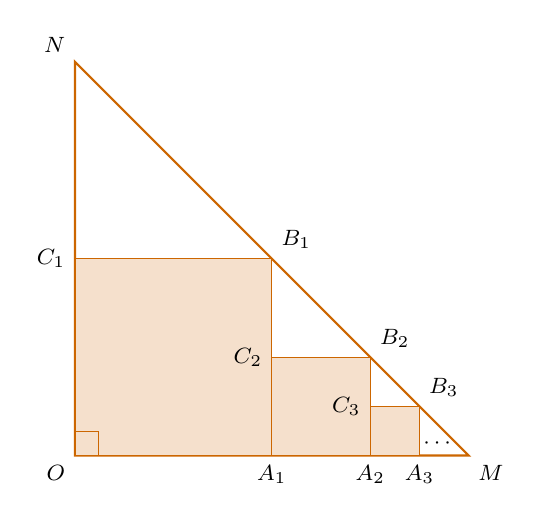
\begin{tikzpicture}
			 \def\a{5}
			\definecolor{customcolor}{rgb}{0.8,0.4,0} 
			 \coordinate (O) at (0,0);
			\coordinate (N) at (0,\a); 
			\coordinate (M) at  (\a,0);
			 \coordinate (A1) at (\a/2,0);
			 \coordinate (B1) at (\a/2,\a/2);
			\coordinate (C1)  at (0,\a/2);
			\coordinate (A2)  at (3*\a/4,0);
			\coordinate (B2)  at (3*\a/4,\a/4);
			\coordinate (C2)  at (\a/2,\a/4);
			 \coordinate (A3) at (7*\a/8,0);
			\coordinate (B3) at (7*\a/8,\a/8); 
			\coordinate (C3) at (3*\a/4,\a/8); 
			\draw[customcolor,thick] (O) --  (N) -- (M) -- cycle;
			\fill[customcolor!20]  (O) rectangle (B1);
			\fill[customcolor!20] (A1) rectangle (B2); 
			\fill[customcolor!20] (A2)  rectangle (B3);
			\draw[customcolor] (O)  rectangle (B1);
			 \draw[customcolor] (A1) rectangle (B2);
			\draw[customcolor] (A2)  rectangle (B3);
			\node[below left]  at (O) {\footnotesize $O$};
			\node[above left] at (N) {\footnotesize  $N$};
			\node[below right] at (M) {\footnotesize $M$}; 
			\node[below] at (A1) {\footnotesize $A_1$}; 
			 \node[below] at (A2) {\footnotesize $A_2$};
			\node[below] at (A3) {\footnotesize $A_3$}; 
			\node[above right] at (B1) {\footnotesize $B_1$}; 
			\node[above right] at  (B2) {\footnotesize $B_2$};
			\node[above right] at (B3)  {\footnotesize $B_3$};
			\node[left] at (C1)  {\footnotesize $C_1$};
			 \node[left] at (C2) {\footnotesize $C_2$};
			\node[left]  at (C3) {\footnotesize $C_3$};
			 \draw[customcolor] (O) ++(0.3,0) -- ++(0,0.3) -- ++(-0.3,0);
			\node at (4.6,0.15)  {\footnotesize $\cdots$};
		\end{tikzpicture}
	} 
	\shortans{0,33} 
	\loigiai{ 
		Độ dài cạnh của các hình vuông lần lượt là $a_1 = \dfrac{1}{2}, a_2 = \left( \dfrac{1}{2}  \right)^2, a_3 = \left( \dfrac{1}{2} \right)^3, \ldots$ \\
		Diện tích của các  hình vuông lần lượt là
		 \[
		S_1 = \left( \dfrac{1}{2} \right)^2 = \dfrac{1}{4}, \quad S_2 = \left( \dfrac{1}{4} \right)^2, \quad S_3 =  \left( \dfrac{1}{4} \right)^3, \ldots
		\] 
		Các diện tích $S_1$, $S_2$,  $S_3$, $\ldots$ tạo thành cấp số nhân lùi vô hạn với số hạng đầu $S_1 = \dfrac{1}{4}$ và công bội $\dfrac{1}{4}$. \\
		Do đó, tổng diện tích các hình vuông  là
		 \[
		S  = \dfrac{1}{4} \cdot \dfrac{1}{1 - \dfrac{1}{4}} = \dfrac{1}{3}
		 \]
	 }
\end{ex}

% nguồn: Ok_TraLoiNgan_Lop11_Lan2
\begin{ex}%[1D3V1-6]%[ma:c15dfdf2]
	Xét dãy các tam giác đều với tam giác đầu tiên có cạnh bằng $3$. Với mỗi số nguyên  dương $n \geq 2$, tam giác sau là tam giác trung bình của tam giác trước. Tính tổng $S$ của diện tích các đường tròn ngoại tiếp dãy tam giác này khi $n \to \infty$.
	 \shortans{42,6}
	\loigiai{ 
		Vì dãy các  tam giác $A_1B_1C_1$, $A_2B_2C_2$, $A_3B_3C_3$, ... là các tam giác đều nên bán kính đường tròn ngoại tiếp các tam giác bằng
		\[\text{cạnh} \cdot \dfrac{\sqrt{3}}{3}.\] 
		Với $n=1$, tam giác đều  $A_1B_1C_1$ có cạnh bằng $3$, nên đường tròn ngoại tiếp tam giác $A_1B_1C_1$ có bán kính
		 \[
		R_1 = 3 \cdot \dfrac{\sqrt{3}}{3} \Rightarrow S_1 = \pi  \left( 3 \cdot \dfrac{\sqrt{3}}{3} \right)^2.
		 \]
		Với $n=2$, tam giác đều  $A_2B_2C_2$ có cạnh bằng $\dfrac{3}{2}$, nên đường tròn ngoại tiếp tam giác $A_2B_2C_2$ có bán kính
		 \[
		R_2 = 3 \cdot \dfrac{1}{2} \cdot \dfrac{\sqrt{3}}{3} \Rightarrow S_2 = \pi \left(  3 \cdot \dfrac{1}{2} \cdot \dfrac{\sqrt{3}}{3} \right)^2.
		 \]
		Với $n=3$, tam giác đều $A_3B_3C_3$ có cạnh bằng $\dfrac{3}{4}$, nên đường tròn ngoại tiếp tam giác $A_3B_3C_3$ có bán  kính
		\[ 
		R_3 = 3 \cdot \dfrac{1}{4} \cdot \dfrac{\sqrt{3}}{3} \Rightarrow S_3 = \pi \left( 3 \cdot  \dfrac{1}{4} \cdot \dfrac{\sqrt{3}}{3} \right)^2.
		\] 
		Như vậy, tam giác đều $A_nB_nC_n$ có cạnh bằng $3 \cdot \left( \dfrac{1}{2} \right)^{n-1}$, nên đường tròn ngoại tiếp tam giác  $A_nB_nC_n$ có bán kính
		\[ 
		 R_n = 3 \cdot \left( \dfrac{1}{2} \right)^{n-1} \cdot \dfrac{\sqrt{3}}{3} \Rightarrow S_n = \pi \left( 3 \cdot \left( \dfrac{1}{2} \right)^{n-1} \cdot \dfrac{\sqrt{3}}{3} \right)^2.
		\] 
		Khi đó, dãy $S_1$, $S_2$, $\dots$, $S_n$, $\dots$ là một cấp số nhân lùi vô hạn với số hạng đầu $u_1  = S_1 = 3\pi$ và công bội $q = \dfrac{1}{4}$.\\
		Do đó, tổng 
		\[ 
		S = S_1 + S_2 + \dots + S_n +  \dots = \dfrac{u_1}{1 - q} = 4\pi \approx 42{,}6.
		\] 
	} 
\end{ex}

% nguồn: Ok_TraLoiNgan_Lop11_Lan2
\begin{ex}%[1D3V1-6]%[ma:abd23042]
	 \immini{
	Từ hình vuông đầu tiên có cạnh bằng $\sqrt{2}$, nối các trung điểm của bốn cạnh để tạo hình vuông tiếp theo. Tính tổng  diện tích $T$ của các hình vuông khi cho số hình vuông tăng lên vô hạn.}
	{ 
	\begin{tikzpicture}
			 \def\a{3}
			 \def\b{0.5}
			 \def\levels{10}
			\coordinate (A0) at  (0,\a);
			\coordinate (B0)  at (\a,2*\a);
			\coordinate (C0)  at (2*\a,\a);
			\coordinate  (D0) at (\a,0);
			\foreach \i in  {1,...,\levels}{
				\coordinate (A\i) at  ($(A\the\numexpr\i-1\relax)!\b!(B\the\numexpr\i-1\relax)$);
				\coordinate (B\i) at ($(B\the\numexpr\i-1\relax)!\b!(C\the\numexpr\i-1\relax)$); 
				\coordinate (C\i)  at ($(C\the\numexpr\i-1\relax)!\b!(D\the\numexpr\i-1\relax)$);
				\coordinate (D\i) at ($(D\the\numexpr\i-1\relax)!\b!(A\the\numexpr\i-1\relax)$); 
				\draw (A\i) -- (B\i) --  (C\i) -- (D\i) -- cycle;
			} 
		\end{tikzpicture}
	} 
	\shortans{4} 
	 \loigiai{
		Ta có $S_1 = \left( \sqrt{2} \right)^2 = 2$, $S_2 =  1$, $S_3 = \dfrac{1}{2}$, $\dots$, $S_n = \dfrac{1}{2^{n-2}}$.\\
		Nhận xét $(S_n)$ là cấp số nhân lùi vô hạn với công bội bằng  $\dfrac{1}{2}$.
		Áp dụng công thức tính tổng cấp số nhân lùi vô hạn ta  có
		 \[
		 T = 2 + 1 + \dfrac{1}{2} + \dfrac{1}{2^2} + \dots + \dfrac{1}{2^{n-2}} + \dots = \dfrac{2}{1 - \dfrac{1}{2}} = 4.
		 \]
	 }
\end{ex}

% nguồn: Ok_TraLoiNgan_Lop11_Lan2
\begin{ex}%[1D3V1-6]%[ma:7fa824c9]
	 \immini{
	Từ một hình vuông có cạnh bằng $1$, người ta nối các trung điểm để tạo  hình vuông mới. Tiếp tục quá trình đến vô hạn, tính tổng diện tích tất cả các hình vuông.
	 }
	 {
	\begin{tikzpicture}
			\def\a{3} 
			 \def\b{0.5}
			\def\levels{10} 
			\coordinate (A0) at (0,\a); 
			\coordinate (B0) at (\a,2*\a); 
			\coordinate (C0) at  (2*\a,\a);
			 \coordinate (D0) at (\a,0);
			 \foreach \i in {1,...,\levels}{
				\coordinate (A\i) at  ($(A\the\numexpr\i-1\relax)!\b!(B\the\numexpr\i-1\relax)$);
				\coordinate  (B\i) at ($(B\the\numexpr\i-1\relax)!\b!(C\the\numexpr\i-1\relax)$);
				\coordinate (C\i) at ($(C\the\numexpr\i-1\relax)!\b!(D\the\numexpr\i-1\relax)$); 
				\coordinate (D\i) at ($(D\the\numexpr\i-1\relax)!\b!(A\the\numexpr\i-1\relax)$); 
				\draw (A\i) --  (B\i) -- (C\i) -- (D\i) -- cycle;
			} 
		\end{tikzpicture}
	} 
	 \shortans{2}
	 \loigiai{
		 Gọi $S_n$ là diện tích của hình vuông thứ $n$.
		Ta có: $S_1 = 1$, $S_2 = \dfrac{1}{2}$, $S_3 = \left( \dfrac{1}{2}  \right)^2$, …
		Dãy $(S_n)$ lập thành  một cấp số nhân với số hạng đầu $S_1 = 1$ và công bội $q = \dfrac{1}{2}$.
		Vì $|q| = \dfrac{1}{2} < 1$, nên $(S_n)$ là một cấp số nhân lùi vô hạn.  \\
		Do đó 
		 \[
		S = 1 + \dfrac{1}{2} + \left(  \dfrac{1}{2} \right)^2 + \left( \dfrac{1}{2} \right)^3 + \dots = \dfrac{1}{1 - \dfrac{1}{2}} = 2.
		 \]
		Vậy tổng diện tích của các hình vuông là $2$. 
	 }
\end{ex}

% nguồn: Ok_TraLoiNgan_Lop11_Lan2
\begin{ex}%[1D3V1-6]%[ma:2086365a]
	Cho hình vuông $C_1$ có cạnh bằng $a$. Người ta chia mỗi cạnh của hình vuông thành bốn phần bằng nhau và nối các điểm  chia một cách thích hợp để có hình vuông $C_2$ (hình vẽ). Từ hình vuông $C_2$ lại tiếp tục làm như trên ta nhận được dãy các hình vuông $C_1$, $C_2$, $C_3$, $\ldots$, $C_n$. Gọi $S_i$ là diện tích của hình vuông $C_i$ $(i \in\{1,2,3, \ldots, n\})$. Khi đó $\lim\limits_{n \to+\infty} \dfrac{2\,025}{a^2}\left(S_1+S_2+\cdots+S_n\right)$ bằng bao nhiêu?
	\begin{center}
		\begin{tikzpicture}[scale=0.8,font=\footnotesize,>=stealth]
				\def\canhAD{6}; 
				\coordinate  (D) at (0,0);
				\coordinate (A)  at ($(D)+(90:\canhAD)$);
				\coordinate (C) at  ($(D)+(0:\canhAD)$);
				\coordinate  (B) at ($(A)+(0:\canhAD)$);
				\coordinate  (E) at ($(A)!0.25!(B)$);
				\coordinate (F) at ($(B)!0.25!(C)$); 
				\coordinate (G) at ($(C)!0.25!(D)$); 
				\coordinate (H) at  ($(D)!0.25!(A)$);
				\coordinate (K)  at ($(E)!0.25!(F)$);
				 \coordinate (L) at ($(F)!0.25!(G)$);
				 \coordinate (M) at ($(G)!0.25!(H)$);
				 \coordinate (J) at ($(H)!0.25!(E)$);
				\coordinate (I) at  ($(E)!0.25!(G)$);
				\coordinate (X) at  ($(J)!0.25!(K)$);
				 \coordinate (Y) at ($(K)!0.25!(L)$);
				\coordinate  (T) at ($(L)!0.25!(M)$);
				\coordinate  (Q) at ($(M)!0.25!(J)$);
				\draw (A) rectangle  (C)
					 (E)--(F)--(G)--(H)--cycle (J)--(K)--(L)--(M)--cycle (X)--(Y)--(T)--(Q)--cycle;
				\draw [>=stealth,|<->|] ([shift=({0,-0.4})]D)--([shift=({0,-0.4})]C) node  [midway,below]{$a$};
			\end{tikzpicture}
	\end{center}
	\shortans{5400} 
	\loigiai{ 
		 Cạnh của hình vuông $C_1$ là $a$. Do đó $S_1=a^2$.\\
		Cạnh của hình  vuông $C_2$ là $\sqrt{\left(\dfrac{3a}{4}\right)^2+\left(\dfrac{a}{4}\right)^2}=\dfrac{a \sqrt{10}}{4}$. Do đó $S_2=\dfrac{10}{16} a^2=\dfrac{10}{16} S_1$.\\
		 Tương tự ta có $S_3=\dfrac{10}{16} S_2$; $\ldots$; $S_n=\dfrac{10}{6} S_{n-1}$.\\
		Khi đó $S_1+S_2+\cdots+S_n=S_1\left[1+\left(\dfrac{10}{16}\right)+\left(\dfrac{10}{16}\right)^2+\left(\dfrac{10}{16}\right)^3+\cdots+\left(\dfrac{10}{16}\right)^{n-1}\right]$.\\ 
		Suy ra 
		\begin{eqnarray*}
			&&\lim\limits_{n \to+\infty} \dfrac{2\,025}{a^2}\left(S_1+S_2+\cdots+S_n\right)\\ 
			&=&\dfrac{2\,025}{a^2} \cdot \dfrac{a^2}{1-\dfrac{10}{16}}\\ 
			&=&\dfrac{2\,025}{a^2} \cdot  \dfrac{8}{3} \cdot a^2\\
			 &=&5\,400.
		\end{eqnarray*}
	 }
\end{ex}

% nguồn: Ok_TraLoiNgan_Lop11_Lan2
\begin{ex}%[1D3V1-6]%[ma:f952fdc7]
	\immini{ 
	Từ hình vuông đầu tiên có cạnh bằng $1$, nối các trung điểm của bốn cạnh để có hình vuông thứ hai. Tiếp tục nối các  trung điểm của bốn cạnh của hình vuông thứ hai để được hình vuông thứ ba. Cứ tiếp tục làm như thế, nhận được một dãy hình vuông.
	Kí hiệu $P_n$ là chu vi của hình vuông thứ $n$ và $Q_n$ là tổng chu vi  của $n$ hình vuông đầu tiên. Tính $\lim Q_n$.
	} 
	{ 
	\begin{tikzpicture}
			\def\a{3} 
			 \def\b{0.5}
			 \def\levels{10}
			 \coordinate (A0) at (0,\a);
			\coordinate  (B0) at (\a,2*\a);
			\coordinate  (C0) at (2*\a,\a);
			\coordinate (D0)  at (\a,0);
			 \foreach \i in {1,...,\levels}{
				 \coordinate (A\i) at ($(A\the\numexpr\i-1\relax)!\b!(B\the\numexpr\i-1\relax)$);
				\coordinate (B\i)  at ($(B\the\numexpr\i-1\relax)!\b!(C\the\numexpr\i-1\relax)$);
				\coordinate  (C\i) at ($(C\the\numexpr\i-1\relax)!\b!(D\the\numexpr\i-1\relax)$);
				\coordinate (D\i) at  ($(D\the\numexpr\i-1\relax)!\b!(A\the\numexpr\i-1\relax)$);
				\draw (A\i)  -- (B\i) -- (C\i) -- (D\i) -- cycle;
			 }
		\end{tikzpicture}
	} 
	 \shortans{8}
	 \loigiai{
		Chu vi $P_n$ của hình vuông lập  thành một cấp số nhân lùi vô hạn với số hạng đầu $u_1=4$ và công bội $q=\dfrac{1}{2}$, có số hạng tổng quát là $P_n = 4 \cdot \left( \dfrac{1}{2} \right)^{n-1}$.\\
		Ta có $Q_n = 4  + 4 \cdot \dfrac{1}{2} + 4 \cdot \dfrac{1}{4} + \ldots + 4 \cdot \left( \dfrac{1}{2} \right)^n + \ldots$\\
		Tổng của cấp số  nhân lùi vô hạn là
		\[ 
		Q = \lim Q_n = 4 \cdot \dfrac{1}{1 -  \dfrac{1}{2}} = 8
		\] 
	} 
\end{ex}

% nguồn: Ok_TraLoiNgan_Lop11_Lan2
\begin{ex}%[1D3V1-6]%[ma:2e4e81f9]
	Từ độ cao $55{,}8$ m của tháp nghiêng Pisa nước Ý, người ta thả một quả bóng cao su chạm xuống đất (hình vẽ). Giả sử mỗi lần chạm đất quả bóng  nảy lên với độ cao bằng $\dfrac{1}{10}$ độ cao mà quả bóng đạt được trước đó. Tổng quãng đường mà quả bóng di chuyển từ khi thả cho đến khi dừng hẳn bằng bao nhiêu mét (kết quả làm tròn đến hàng phần chục)?
	 \definecolor{lightcornflowerblue}{rgb}{0.6, 0.81, 0.93}
	\definecolor{cadmiumgreen}{rgb}{0.0, 0.42, 0.24} 
	\definecolor{trueblue}{rgb}{0.0, 0.45,  0.81}
	\definecolor{tumbleweed}{rgb}{0.87, 0.67, 0.53} 
	\begin{center}
		\begin{tikzpicture}[line join=round,line cap=round,scale=0.7,transform shape]
				\clip  (-4,-3.5) rectangle (4,3.5);
				 \tikzset{thap/.pic={
				 \def\T{
					(-.88,-1.78) 
					..controls +(40:.17) and  +(120:.1).. (.686,-1.91)--(.68,-1.94)
					..controls +(120:.1) and  +(40:.12).. (-.87,-1.81)
					--cycle 
					(-.8,-1.2) 
					..controls +(40:.14) and +(120:.14)..  (.72,-1.34)--(.7,-1.36)
					..controls +(120:.1) and +(40:.12)..  (-.78,-1.23)
					--cycle 
					(-.74,-.65) 
					..controls +(40:.22) and  +(120:.17).. (.74,-.78)--(.72,-.8)
					..controls +(120:.15)  and +(40:.15).. (-.72,-.67)
					--cycle 
					 (-.68,-.13)
					 ..controls +(40:.34) and +(110:.2).. (.8,-.26)--(.78,-.28)
					..controls  +(110:.17) and +(40:.27).. (-.66,-.15)
					--cycle 
					(-.65,.36) 
					..controls +(40:.44) and +(120:.3).. (.85,.24)--(.83,.22) 
					..controls +(130:.35) and +(40:.35)..  (-.63,.34)
					--cycle 
					(-.58,.88) 
					..controls +(40:.44) and  +(120:.3).. (.87,.78)--(.85,.76)
					..controls +(130:.35) and +(40:.35)..  (-.56,.86)
					--cycle 
					 (-.52,1.35)
					..controls  +(120:.32) and +(110:.47).. (.93,1.26)--(.9,1.25)
					..controls +(110:.43) and +(110:.27).. (-.49,1.35) 
					--cycle 
					 (-.31,2)
					..controls +(120:.47) and +(55:.46)..  (.76,1.94)--(.74,1.94)
					..controls +(75:.31) and +(115:.28).. (-.28,2) 
					--cycle 
					 (-.48,1.5)
					..controls +(40:.33) and +(110:.2)..  (.86,1.4)
					(-.476,1.52) 
					..controls +(40:.33)  and +(110:.2).. (.86,1.42)
					(-.472,1.54) 
					..controls  +(40:.33) and +(110:.2).. (.86,1.44)
					(-.468,1.56) 
					..controls +(40:.33) and  +(110:.2).. (.86,1.46)
					 (-.28,2.2)
					..controls +(40:.27) and +(140:.2)..  (.74,2.16)
					 (-.276,2.22)
					..controls +(40:.27) and  +(140:.2).. (.74,2.18)
					(-.272,2.24) 
					 ..controls +(40:.27) and +(140:.2).. (.74,2.2)
					(-.268,2.26) 
					 ..controls +(40:.27) and +(140:.2).. (.74,2.22);}
				 \draw \T;
					 }}
				 \tikzset{rao/.pic={
				\def\R{ 
					 (-.48,1.5)
					..controls +(40:.33) and +(110:.2).. (.86,1.4) 
					(-.476,1.52) 
					..controls +(40:.33) and  +(110:.2).. (.86,1.42)
					(-.472,1.54) 
					..controls +(40:.33) and +(110:.2)..  (.86,1.44)
					(-.468,1.56) 
					..controls +(40:.33) and  +(110:.2).. (.86,1.46)
					 (-.28,2.2)
					..controls +(40:.27) and +(140:.2)..  (.74,2.16)
					 (-.276,2.22)
					..controls +(40:.27) and  +(140:.2).. (.74,2.18)
					 (-.272,2.24)
					..controls +(40:.27)  and +(140:.2).. (.74,2.2)
					(-.268,2.26) 
					 ..controls +(40:.27) and +(140:.2).. (.74,2.22);}
				\draw  \R;
					 }}
				\tikzset{co/.pic={ 
				\def\C{ 
					(0.1,2.3)--(.1,2.9) 
					(.1,2.82) 
					..controls  +(-40:.2) and +(140:.22).. (.2,2.6)
					..controls +(-60:0) and  +(100:.1)..(.16,2.5)
					..controls +(140:.1) and +(-30:0)..  (.1,2.53)--cycle;}
				 \draw \C;
				 \fill[red] \C;
					 }}
				 \tikzset{cong0/.pic={
				 \def\D0{
					 (.68,-1.96)
					 ..controls +(120:.1) and +(40:.12).. (-.87,-1.81)--
					(-.87,-1.94) 
					..controls +(80:.12) and  +(95:0.12).. (-.68,-2.06)
					..controls  +(80:.12) and +(85:0.3).. (-.4,-2.12)
					..controls +(80:.25) and +(95:0.25).. (-.02,-2.12) 
					..controls +(80:.25) and +(95:0.25)..  (.27,-2.14)
					..controls  +(80:.12) and +(95:0.12).. (.5,-2.14)
					..controls +(70:.12) and +(95:0.02)..  (.66,-2.1)--cycle;}
				\draw  \D0;
				\fill[tumbleweed] \D0; 
					}} 
				 \tikzset{cong1/.pic={
				 \def\D1{
					 (.7,-1.36)
					..controls +(120:.1)  and +(40:.12).. (-.78,-1.23)--
					(-.78,-1.35) 
					..controls +(80:.12) and  +(95:0.12).. (-.72,-1.35)
					..controls +(80:.12) and  +(95:0.12).. (-.64,-1.35)
					..controls +(80:.12) and +(95:0.12)..  (-.55,-1.35)
					 ..controls +(80:.12) and +(95:0.12).. (-.44,-1.36)
					..controls +(80:.12) and +(95:0.12).. (-.3,-1.37) 
					..controls +(80:.12) and  +(95:0.12).. (-.14,-1.38)
					..controls +(80:.12)  and +(95:0.12).. (0.02,-1.39)
					..controls +(80:.12) and +(95:0.12)..  (0.18,-1.4)
					..controls +(80:.12)  and +(95:0.12).. (0.32,-1.42)
					..controls +(70:.12) and +(95:0.12)..  (0.42,-1.44)
					 ..controls +(70:.12) and +(95:0.12).. (0.52,-1.46)
					..controls +(70:.12) and  +(95:0.12).. (0.6,-1.47)
					..controls +(70:.12) and +(95:0.12)..  (0.68,-1.5)--cycle;}
				\draw  \D1;
				\fill[tumbleweed]  \D1;
					}} 
				\tikzset{cong2/.pic={ 
				 \def\D2{
					 (.72,-.8)
					..controls +(120:.15) and +(40:.15).. (-.72,-.67)-- 
					 (-.72,-.79)
					..controls  +(80:.12) and +(95:0.12).. (-.66,-.79)
					..controls +(80:.12) and +(95:0.12)..  (-.58,-.79)
					..controls +(80:.12) and +(95:0.12).. (-.48,-.79) 
					..controls +(80:.12)  and +(95:0.12).. (-.38,-.8)
					..controls +(80:.12) and  +(95:0.12).. (-.23,-.8)
					..controls +(80:.12) and  +(95:0.12).. (-0.08,-.81)
					..controls +(80:.12) and +(95:0.12)..  (0.08,-.82)
					..controls +(80:.12)  and +(95:0.12).. (0.22,-.84)
					..controls +(80:.12) and +(95:0.12).. (0.36,-.85) 
					..controls +(70:.12) and +(95:0.12).. (0.48,-.87) 
					..controls  +(70:.12) and +(95:0.12).. (0.58,-.89)
					..controls +(70:.12)  and +(95:0.12).. (0.66,-.9)
					..controls +(70:.12) and +(95:0.12)..  (0.71,-.92)--cycle;}
				\draw  \D2;
				 \fill[tumbleweed] \D2;
					}} 
				 \tikzset{cong3/.pic={
				\def\D3{ 
					(.78,-.28) 
					..controls +(110:.17) and  +(40:.27).. (-.66,-.15)--
					(-.66,-.26) 
					..controls +(80:.12) and +(95:0.12).. (-.6,-.25) 
					..controls +(80:.12)  and +(95:0.12).. (-.52,-.24)
					..controls +(80:.12) and  +(95:0.12).. (-.44,-.23)
					..controls +(80:.12) and +(95:0.12).. (-.32,-.23) 
					..controls +(80:.12)  and +(95:0.12).. (-.18,-.23)
					..controls +(80:.12)  and +(95:0.12).. (-.04,-.24)
					..controls +(80:.12) and +(95:0.12).. (0.13,-.25) 
					 ..controls +(80:.12) and +(95:0.12).. (0.26,-.26)
					 ..controls +(70:.12) and +(95:0.12).. (0.42,-.29)
					..controls +(70:.12)  and +(95:0.12).. (0.54,-.31)
					..controls +(70:.12) and +(95:0.12)..  (0.63,-.33)
					 ..controls +(70:.12) and +(95:0.12).. (0.7,-.35)
					 ..controls +(70:.12) and +(95:0.12).. (0.765,-.38)--cycle;}
				\draw  \D3;
				\fill[tumbleweed]  \D3;
					 }}
				 \tikzset{cong4/.pic={
				 \def\D4{
					(.83,.22) 
					..controls +(130:.35)  and +(40:.35).. (-.63,.34)--
					(-.63,.23) 
					..controls +(80:.12) and +(95:0.12)..  (-.57,.25)
					 ..controls +(80:.12) and +(95:0.12).. (-.49,.26)
					 ..controls +(80:.12) and +(95:0.12).. (-.4,.28)
					..controls +(80:.12)  and +(95:0.12).. (-.27,.3)
					..controls +(80:.12) and +(95:0.12)..  (-.15,.3)
					..controls  +(80:.12) and +(95:0.12).. (0.02,.3)
					..controls +(80:.12) and  +(95:0.12).. (0.16,.29)
					..controls +(80:.12) and  +(95:0.12).. (0.31,.27)
					..controls +(70:.12) and  +(95:0.12).. (0.45,.25)
					 ..controls +(70:.12) and +(95:0.12).. (0.58,.23)
					..controls +(70:.12) and +(95:0.12)..  (0.67,.2)
					 ..controls +(70:.12) and +(95:0.12).. (0.75,.17)
					..controls  +(70:.12) and +(95:0.12).. (0.8,.14)--cycle;}
				\draw  \D4;
				 \fill[tumbleweed] \D4;
					}} 
				 \tikzset{cong5/.pic={
				 \def\D5{
					 (.85,.76)
					 ..controls +(130:.35) and +(40:.35).. (-.56,.86)--
					 (-.56,.74)
					..controls +(80:.12) and +(95:0.12).. (-.5,.77) 
					 ..controls +(80:.12) and +(95:0.12).. (-.44,.79)
					..controls  +(80:.12) and +(95:0.12).. (-.34,.81)
					..controls  +(80:.12) and +(95:0.12).. (-.22,.83)
					..controls +(80:.12) and  +(95:0.12).. (-0.08,.85)
					 ..controls +(80:.12) and +(95:0.12).. (0.06,.85)
					..controls +(80:.12) and +(95:0.12).. (0.22,.83) 
					..controls +(70:.12)  and +(95:0.12).. (0.36,.81)
					 ..controls +(70:.12) and +(95:0.12).. (0.5,.78)
					..controls +(70:.12) and +(95:0.12)..  (0.62,.74)
					..controls +(70:.12)  and +(95:0.12).. (0.73,.72)
					..controls  +(70:.12) and +(95:0.12).. (0.82,.68)--cycle;}
				\draw \D5; 
				\fill[tumbleweed] \D5; 
					 }}
				\tikzset{cong6/.pic={ 
				\def\D6{ 
					 (.9,1.25)
					..controls +(110:.43)  and +(110:.27).. (-.49,1.35)--
					(-.49,1.3) 
					..controls +(80:.12) and  +(95:0.12).. (-.45,1.33)
					..controls  +(80:.12) and +(95:0.12).. (-.38,1.33)
					..controls +(80:.12) and +(95:0.12).. (-.28,1.35) 
					..controls +(80:.12) and +(95:0.12)..  (-.16,1.37)
					..controls +(80:.12) and  +(95:0.12).. (-0.04,1.38)
					..controls  +(80:.12) and +(95:0.12).. (0.12,1.38)
					..controls +(80:.12) and  +(95:0.12).. (0.26,1.38)
					..controls +(70:.12)  and +(95:0.12).. (0.42,1.37)
					..controls +(70:.12) and +(95:0.12)..  (0.55,1.34)
					..controls  +(70:.12) and +(95:0.12).. (0.67,1.3)
					 ..controls +(70:.12) and +(95:0.12).. (0.78,1.25)
					..controls +(70:.12) and +(95:0.12)..  (0.84,1.21)
					..controls +(70:.12) and  +(95:0.12).. (0.88,1.16)--cycle;}
				 \draw \D6;
				\fill[tumbleweed]  \D6;
					}} 
				\tikzset{cong7/.pic={ 
				\def\D7{ 
					(.74,1.94) 
					..controls +(75:.31) and  +(115:.28).. (-.28,2)--
					(-.28,1.94) 
					..controls  +(80:.12) and +(95:0.12).. (-.24,1.98)
					..controls +(80:.12) and +(95:0.12)..  (-.14,2.04)
					 ..controls +(80:.12) and +(95:0.12).. (0.02,2.08)
					 ..controls +(80:.12) and +(95:0.12).. (0.2,2.08)
					..controls +(80:.12) and +(95:0.12).. (0.4,2.05) 
					..controls +(80:.12) and  +(95:0.12).. (0.56,2)
					 ..controls +(80:.12) and +(95:0.12).. (0.66,1.96)
					..controls +(70:.12) and +(95:0.12).. (0.74,1.9)--cycle;} 
				\draw \D7; 
				 \fill[tumbleweed] \D7;
					}} 
				 \tikzset{cua/.pic={
				 \def\W{
					 (-.7,-2.85)--(-.63,-2.25)
					..controls +(70:.1) and +(100:.1)..  (-.46,-2.25)--(-.52,-2.85)
					--cycle;} 
				\draw \W; 
				\fill[tumbleweed]  \W;
					}} 
				\tikzset{vien/.pic={ 
				\def\V{ 
					 (.9,1.25)
					 ..controls +(110:.43) and +(110:.27).. (-.49,1.35)--(-.98,-2.85)--(.59,-2.85)--cycle
					 (.74,1.94)
					..controls +(75:.31) and +(115:.28).. (-.28,2)--(-.32,1.54) 
					..controls  +(115:.2) and +(75:.13).. (.72,1.48)--cycle;}
				 \draw \V;
				\fill[gray!50!]  \V;
					 }}
				\tikzset{soc/.pic={ 
				 \def\S{
					(.82,1.36)--(.54,-1.85)--(.58,-1.85)--(.86,1.36) 
					 --cycle;}
				\draw  \S;
				\fill[tumbleweed!40!]  \S;
					 }}
				 \tikzset{soc2/.pic={
				\def\S{ 
					(.54,-1.95)--(.44,-2.85)--(.48,-2.85)--(.58,-1.95) 
					--cycle;} 
				\draw  \S;
				\fill[tumbleweed!40!]  \S;
					}} 
				\tikzset{soc3/.pic={ 
				 \def\S{
					(.54,2)--(.57,2)--(.54,1.5)--(.51,1.5) 
					--cycle 
					(.66,2)--(.69,2)--(.66,1.5)--(.63,1.5) 
					 --cycle
					 (-.26,2)--(-.23,2)--(-.26,1.5)--(-.29,1.5)
					 --cycle;}
				 \draw \S;
				 \fill[tumbleweed!40!] \S;
					}} 
				 \tikzset{thoi/.pic={
				 \def\T{
					(0.15,-1.98)--(.24,-2.12)--(0.13,-2.22)--(0.04,-2.1) 
					--cycle;} 
				\draw  \T;
				\fill[tumbleweed!40!]  \T;
					 }}
				\tikzset{cay/.pic={ 
				\def\T{ 
					 (-1.73,-2.85)
					..controls +(40:.03) and +(40:.01)..  (-1.74,-2.7)
					 ..controls +(140:.04) and +(60:.02).. (-1.78,-2.6)
					..controls  +(140:.04) and +(60:.02).. (-1.8,-2.55)
					..controls +(100:.03) and  +(70:.02).. (-1.82,-2.5)
					..controls +(140:.04) and  +(60:.02).. (-1.815,-2.4)
					 ..controls +(140:.04) and +(60:.02).. (-1.818,-2.3)
					 ..controls +(85:.03) and +(-30:.03).. (-1.8,-2.2)
					..controls +(80:.04) and  +(50:.02).. (-1.78,-2)
					..controls  +(60:.04) and +(120:.02).. (-1.76,-1.9)
					..controls +(80:.03) and  +(-100:.02).. (-1.74,-1.8)
					..controls  +(80:.01) and +(-100:.02).. (-1.72,-1.9)
					..controls  +(60:.02) and +(-120:.02).. (-1.7,-2)
					..controls +(-80:.02) and  +(110:.03).. (-1.66,-2.2)
					..controls +(-100:.02)  and +(60:.03).. (-1.64,-2.3)
					..controls +(-30:.02) and +(70:.02).. (-1.6,-2.44) 
					 ..controls +(-100:.02) and +(70:.02).. (-1.63,-2.52)
					..controls +(-60:.02) and +(70:.01)..  (-1.66,-2.6)
					..controls +(60:.01) and +(70:.02)..  (-1.7,-2.7)
					 ..controls +(-120:.02) and +(120:.03).. (-1.68,-2.85);}
				\draw \T; 
				\fill[cadmiumgreen!90!]  \T;
					}} 
				 \fill[cadmiumgreen!80!] (-4,-3.5) rectangle (8,-2.2);
				\fill[lightcornflowerblue]  (-4,3.5) rectangle (8,-2.2);
				 \path
					(0,0)  pic[scale=1]{cay}
					(.35,0)  pic[scale=.9]{cay}
					(1.05,0.6) pic[scale=1.2]{cay} 
					(-.5,-1) pic[scale=.6]{cay} 
					(3,0)  pic[scale=1]{cay}
					(2.8,0)  pic[scale=1]{cay}
					(0,0) pic[scale=1]{vien} 
					(0,0)  pic[scale=1]{soc}
					 (0,0) pic[scale=1]{soc}
					(-.15,0)  pic[scale=1]{soc}
					 (-.3,0) pic[scale=1]{soc}
					(-.45,0) pic[scale=1]{soc} 
					(-.6,0)  pic[scale=1]{soc}
					(-.75,0) pic[scale=1]{soc} 
					(-.9,0) pic[scale=1]{soc} 
					 (-1.02,0) pic[scale=1]{soc}
					(-1.12,0) pic[scale=1]{soc} 
					 (-1.22,0) pic[scale=1]{soc}
					 (-1.32,0) pic[scale=1]{soc}
					(0,0) pic[scale=1]{soc3} 
					(0,0) pic[scale=1]{thap} 
					 (0,0) pic[scale=1]{co}
					(.4,3.6)  pic[scale=.7,rotate=3]{cua}
					 (.8,3.6) pic[scale=1.2,rotate=7,yscale=.6]{cua}
					(.3,3.4)  pic[scale=1.1,rotate=7,yscale=.6]{cua}
					 (0,-.04) pic[scale=1]{thoi}
					 (0.25,-.05) pic[scale=1]{thoi}
					(-0.35,0) pic[scale=1]{thoi} 
					(-.67,0) pic[scale=1]{thoi} 
					 (-.9,0) pic[scale=1]{thoi}
					(-1.22,0) pic[scale=1]{soc2} 
					(-1.36,0)  pic[scale=1]{soc2}
					 (-.94,0) pic[scale=1]{soc2}
					 (-.56,0) pic[scale=1]{soc2}
					 (-.56,0) pic[scale=1]{soc2}
					(.08,0) pic[scale=1]{soc2} 
					(-.04,0)  pic[scale=1]{soc2}
					(-.28,0)  pic[scale=1]{soc2}
					(0,0) pic[scale=1]{cong0} 
					(0,0.02) pic[scale=1]{cong0} 
					(0,0)  pic[scale=1]{cong1}
					 (0,0.02) pic[scale=1]{cong1}
					(0,0) pic[scale=1]{cong2} 
					(0,0.02)  pic[scale=1]{cong2}
					(0,0) pic[scale=1]{cong3} 
					 (0,0.02) pic[scale=1]{cong3}
					(0,0)  pic[scale=1]{cong4}
					 (0,0.02) pic[scale=1]{cong4}
					 (0,0) pic[scale=1]{cong5}
					(0,0.02)  pic[scale=1]{cong5}
					(0,0) pic[scale=1]{cong6} 
					 (0,0.02) pic[scale=1]{cong6}
					 (0,0) pic[scale=1]{cong7}
					 (0,0.02) pic[scale=1]{cong7}
					(0,0) pic[scale=1]{cua} 
					 (0,0) pic[scale=1]{rao};
			\end{tikzpicture}
	\end{center}
	 \shortans{68,2}
	\loigiai{ 
		Quãng đường đầu tiên bóng rơi  xuống chạm đất lần $1$ là $55{,}8$ m.\\
		Quãng đường nảy lên  lần thứ nhất và rơi xuống chạm đất lần $2$ là $2\cdot \dfrac{55{,}8}{10}$ (m).\\
		Quãng đường nảy  lên lần thứ hai và rơi xuống chạm đất lần $3$ là $2\cdot \dfrac{55{,}8}{10^2}$ (m).\\
		Quãng đường nảy lên lần thứ ba và rơi xuống chạm đất lần thứ $4$ là $2\cdot  \dfrac{55{,}8}{10^3}$ (m).\\
		Vậy nếu gọi $S_n$ là tổng độ dài quãng đường di chuyển của quả bóng tính từ lúc thả ban đầu cho đến khi quả bóng nảy lên lần thứ $n$ rồi chạm đất thì khi đó ta có 
		\begin{eqnarray*}
			S_n&=&55{,}8+2\cdot55{,}8\left(\dfrac{1}{10}+\dfrac{1}{10^2}+\ldots+\dfrac{1}{10^n}\right)\\ 
			&=&55{,}8\left(1+2\left(\dfrac{1}{10}+\dfrac{1}{10^2}+\ldots+\dfrac{1}{10^n}\right)\right)\\ 
			 &=&55{,}8\left(1+\dfrac{2}{9}\left(1-\left(\dfrac{1}{10}\right)^n\right)\right) \, \text{ (m)}.
		\end{eqnarray*}
		Do đó tổng quãng đường mà quả bóng di chuyển  từ khi thả cho đến khi dừng hẳn là
		\begin{eqnarray*}
			S&=&\lim S_n\\ 
			 &=&\lim \left(55{,}8\left(1+\dfrac{2}{9}\left(1-\left(\dfrac{1}{10}\right)^n\right)\right)\right)\\
			&=&55{,}8\left(1+\dfrac{2}{9}\right) \approx  68{,}2\, \text{ (m)}.
		\end{eqnarray*}
	} 
\end{ex}

% nguồn: Ok_TraLoiNgan_Lop11_Lan2
\begin{ex}%[1D3V1-6]%[ma:a46f4166]
	Người ta làm lỗ thông gió của một ngôi nhà bằng cách ghép một dãy hình tròn có cùng bán kính là $0{,}03$\,m. Kí hiệu $u_n$ là tổng diện tích hình tròn ghép được ở bước thứ $n$. Tìm $u_{1\,000}$ (kết quả  làm tròn đến hàng đơn vị).
	\begin{center}
		\begin{tikzpicture}[scale=0.8]
				\shade[top color=gray!15,bottom color=gray!85]  (0,0) rectangle (1,1);
				\filldraw[fill=white]  (0.5,0.5) circle (0.3);
				\node  at (0.5,-0.5) {Bước 1};
				\shade[top color=gray!15,bottom color=gray!85] (3,0) rectangle  (5,2);
				\foreach \i in {0,1}{ 
					\foreach  \j in {0,1}{
					\filldraw[fill=white] (\i+3.5,\j+0.5) circle (0.3); 
				 }
				 }
				\node at (4,-0.5)  {Bước 2};
				\shade[top color=gray!15,bottom color=gray!85] (7,0)  rectangle (10,3);
				\foreach \i in  {0,1,2}{
					 \foreach \j in {0,1,2}{
					\filldraw[fill=white] (\i+7.5,\j+0.5) circle (0.3); 
				 }
				 }
				\node at (8.5,-0.5)  {Bước 3};
				\shade[top color=gray!15,bottom color=gray!85]  (12,0) rectangle (18,6);
				\foreach \i in  {0,1,2,3}{
					\filldraw[fill=white]  (\i+12.5,0.5) circle (0.3);
				 }
				\node  at (16.5,0.5) {$\dots$};
				\node at  (14.5,-0.5) {Bước... Bước $n$};
			\end{tikzpicture}
	\end{center}
	 \shortans{2,83}
	 \loigiai{
		 Ta có
		 \[
		u_1 = \pi \cdot 3^2, \quad u_2 = 4 \cdot \pi  \cdot 3^2, \quad u_3 = 9 \cdot \pi \cdot 3^2, \quad \ldots, \quad u_n = n^2 \cdot \pi \cdot 3^2
		\] 
		Suy ra $u_{1\,000} = 1\,000^2 \cdot \pi  \cdot 0{,}03^2$. \\
		 Vậy $u_{1\,000} = 900\pi \approx 2\,827$\,m$^2$.
	} 
\end{ex}

% nguồn: Ok_TraLoiNgan_Lop11_Lan2
\begin{ex}%[1D3V1-6]%[ma:9958b81f]
	Người ta làm lỗ thông gió của một ngôi nhà bằng cách ghép một dãy hình tròn có cùng bán kính là $3$\,cm. Kí hiệu $u_n$ là tổng diện tích hình tròn ghép được  ở bước thứ $n$. Tìm $n$ nhỏ nhất để $u_n$ vượt quá $9\pi$\,m$^2$.
	\begin{center}
		\begin{tikzpicture}[scale=0.8]
				\shade[top color=gray!15,bottom color=gray!85] (0,0)  rectangle (1,1);
				\filldraw[fill=white] (0.5,0.5) circle (0.3); 
				\node at  (0.5,-0.5) {Bước 1};
				\shade[top  color=gray!15,bottom color=gray!85] (3,0) rectangle (5,2);
				\foreach \i in {0,1}{ 
					\foreach \j  in {0,1}{
					\filldraw[fill=white] (\i+3.5,\j+0.5) circle  (0.3);
				 }
				 }
				\node at (4,-0.5)  {Bước 2};
				\shade[top color=gray!15,bottom  color=gray!85] (7,0) rectangle (10,3);
				\foreach  \i in {0,1,2}{
					\foreach \j in  {0,1,2}{
					\filldraw[fill=white]  (\i+7.5,\j+0.5) circle (0.3);
				 }
				 }
				\node at (8.5,-0.5)  {Bước 3};
				\shade[top color=gray!15,bottom color=gray!85] (12,0) rectangle (18,6); 
				 \foreach \i in {0,1,2,3}{
					\filldraw[fill=white] (\i+12.5,0.5) circle (0.3); 
				} 
				\node at (16.5,0.5)  {$\dots$};
				 \node at (14.5,-0.5) {Bước... Bước $n$};
			\end{tikzpicture}
	\end{center}
	\shortans{101} 
	 \loigiai{
		Ta  có
		\[ 
		u_1 = \pi \cdot 3^2, \quad u_2 = 4 \cdot \pi \cdot 3^2, \quad u_3 = 9 \cdot \pi \cdot 3^2, \quad \ldots, \quad u_n =  n^2 \cdot \pi \cdot 3^2
		\] 
		Xét $u_n > 90\,000 \pi \Rightarrow n^2 > 10\,000 \Rightarrow n  > 100$. \\
		Vậy $n = 101$ là giá trị nhỏ nhất để $u_n$ vượt quá  $90\,000\pi$.
	 }
\end{ex}

% nguồn: Ok_TraLoiNgan_Lop11_Lan2
\begin{ex}%[1D3V1-6]%[ma:d7cb396c]
	Có $1$ kg chất phóng xạ độc hại. Biết rằng, cứ sau một khoảng thời gian $T=24\,000$ năm thì một nửa số chất phóng xạ này bị phân rã thành chất khác không độc hại đối với sức khoẻ của con người. Gọi $u_n$ là khối lượng chất phóng xạ còn lại sau chu kì thứ $n$. Biết rằng sau một số năm nào đó khối lượng chất phóng xạ đã cho ban đầu không còn độc hại  đối với con người, biết rằng chất phóng xạ này sẽ không độc hại nữa nếu khối lượng chất phóng xạ còn lại bé hơn $10^{-6}$\,g. Tìm số chu kì bé nhất để chất phóng xạ đã cho ban đầu không còn độc hại đối với con người.
	 \shortans{31}
	 \loigiai{
		Ta có $u_1=1$, $u_2=\dfrac{1}{2}$, $u_3=\left( \dfrac{1}{2} \right)^2,  \ldots$.\\
		Suy ra  $( u_n)$ lập thành một cấp số nhân có số hạng đầu $u_1=1$ và $q=\dfrac{1}{2}$, với số hạng tổng quát là $u_n=\left( \dfrac{1}{2} \right)^{n-1}$.\\
		Đổi  $u_n = \left( \dfrac{1}{2} \right)^{n-1} \times 10^3$\,g.\\
		Để chất phóng xạ bé hơn $10^{-6}$\,g thì $\left( \dfrac{1}{2} \right)^{n-1} \cdot 10^3 < 10^{-6}  \Rightarrow n > 30$.\\
		Vậy  cần ít nhất $31$ chu kì, tương ứng với $744\,000$ năm, để khối lượng chất phóng xạ ban đầu không còn độc hại.
	 }
\end{ex}

% nguồn: Ok_TraLoiNgan_Lop11_Lan2
\begin{ex}%[1D3C1-6]%[ma:ac26a266]
	\immini{ 
	Cho hình vuông $C_1$ có cạnh bằng $4$. Người ta chia mỗi cạnh thành $4$ phần bằng nhau và nối các điểm chia để tạo hình vuông $C_2$. Tiếp tục quá trình này, tính tổng diện tích của các hình vuông  (kết quả làm tròn đến hàng phần mười).
	} 
	{\begin{tikzpicture}
		 \def\a{3}
		\def\b{0.25} 
		\def\levels{10} 
		 \coordinate (A0) at (0,0);
		\coordinate (B0)  at (\a,0);
		 \coordinate (C0) at (\a,\a);
		\coordinate  (D0) at (0,\a);
		\foreach \i in  {1,...,\levels}{
			\coordinate (A\i) at ($(A\the\numexpr\i-1\relax)!\b!(B\the\numexpr\i-1\relax)$); 
			\coordinate (B\i)  at ($(B\the\numexpr\i-1\relax)!\b!(C\the\numexpr\i-1\relax)$);
			\coordinate  (C\i) at ($(C\the\numexpr\i-1\relax)!\b!(D\the\numexpr\i-1\relax)$);
			\coordinate (D\i)  at ($(D\the\numexpr\i-1\relax)!\b!(A\the\numexpr\i-1\relax)$);
			\draw (A\i) --  (B\i) -- (C\i) -- (D\i) -- cycle;
		 }
	\end{tikzpicture}
	} 
	\shortans{42,6} 
	 \loigiai{
		Gọi  hình vuông $C_1$ có cạnh $a_1 = 4$ và có diện tích là $S_1 = a_1^2$.\\
		Cạnh của hình vuông $C_2$  là
		\[ 
		a_2 = \sqrt{\left( \dfrac{3}{4} a_1 \right)^2 + \left( \dfrac{1}{4} a_1 \right)^2} = \dfrac{a_1 \sqrt{10}}{4}. 
		 \]
		Diện tích của  hình vuông $C_2$ là
		 \[
		 S_2 = \dfrac{5}{8} a_1^2 = \dfrac{5}{8} S_1.
		 \]
		 Cạnh của hình vuông $C_3$ là
		\[ 
		a_3 = \sqrt{\left( \dfrac{3}{4} a_2 \right)^2 + \left( \dfrac{1}{4}  a_2 \right)^2} = \dfrac{a_2 \sqrt{10}}{4} = a_1 \left( \dfrac{\sqrt{10}}{4} \right)^2.
		 \]
		 Diện tích của hình vuông $C_3$ là
		\[ 
		S_3 = \left( \dfrac{5}{8}  \right)^2 a_1^2 = \left( \dfrac{5}{8} \right)^2 S_1.
		\] 
		Lý luận tương tự, ta có dãy các hình vuông $C_1$, $C_2$, $C_3$, $\dots$, $C_n$, $\dots$ có các diện tích lần lượt là $S_1$, $S_2$, $S_3$, $\dots$, $S_n$, $\dots$ tạo thành một cấp số nhân lùi vô hạn với số hạng đầu là $u_1 = S_1 =  16$ và công bội $q = \dfrac{5}{8}$.\\
		Vậy tổng diện tích của  các hình vuông là
		\[ 
		S = S_1 + S_2 + S_3 + \dots + S_n + \dots = \dfrac{u_1}{1 -  q} = \dfrac{16}{1 - \dfrac{5}{8}} = \dfrac{128}{3} \approx 42{,}6.
		\] 
	 }
\end{ex}

% nguồn: Ok_TraLoiNgan_Lop11_Lan2
\begin{ex}%[1D3C1-6]%[ma:f75f3ed6]
	Một bệnh nhân hàng ngày phải uống một viên  thuốc $192$\,mg. Sau ngày đầu, trước mỗi lần uống, hàm lượng thuốc cũ trong cơ thể vẫn còn $4\%$ lượng thuốc của ngày hôm trước. Tính lượng thuốc có trong cơ thể sau khi uống viên thuốc của ngày thứ $3$. Ước tính lượng thuốc trong cơ thể nếu bệnh nhân sử dụng thuốc trong một thời gian dài (kết quả làm tròn đến hàng đơn vị).
	 \shortans{208}
	 \loigiai{
		Gọi $u_n$ là lượng  thuốc trong cơ thể bệnh nhân sau $n$ ngày dùng thuốc.\\
		Ta có $u_1 = 200$. Từ đó, $u_2 = u_1 \cdot \dfrac{1}{25} + 200 = 208$, $u_3  = u_2 \cdot \dfrac{1}{25} + 200 = 208{,}32$,... \\
		Tổng quát,  $u_n = u_{n-1} \cdot \dfrac{1}{25} + 200, n \geq 2$. \\
		 Ta có
		 \[
		u_n -  \dfrac{625}{3} = \dfrac{1}{25} \left( u_{n-1} - \dfrac{625}{3} \right)
		\] 
		Xét dãy $\{ v_n \}$ với $v_n = u_n - \dfrac{625}{3}$. Do $\dfrac{v_n}{v_{n-1}} = \dfrac{1}{25}$, nên $\{ v_n \}$ là cấp  số nhân lùi vô hạn. \\
		Do đó $\lim_{n \to +\infty} v_n = 0 \Rightarrow \lim_{n \to +\infty}  u_n = \dfrac{625}{3} \approx 208$. \\
		Vậy lượng  thuốc trong cơ thể nếu bệnh nhân sử dụng thuốc trong một thời gian dài là $208$\,mg.
	 }
\end{ex}

% nguồn: Ok_TraLoiNgan_Lop11_Lan2
\begin{ex}%[1D3C1-6]%[ma:b7da4026]
	Từ tờ giấy, cắt một hình tròn bán kính $R=10$\,cm. Tiếp theo, cắt hai hình tròn bán kính $\dfrac{R}{2}$ chồng lên hình tròn đầu tiên. Tiếp tục cắt bốn hình tròn bán kính $\dfrac{R}{4}$ và chồng lên các hình trước, tiếp tục quá trình này mãi mãi. Tính tổng diện tích của các  hình tròn (kết quả làm tròn đến hàng đơn vị).
	\begin{center}
		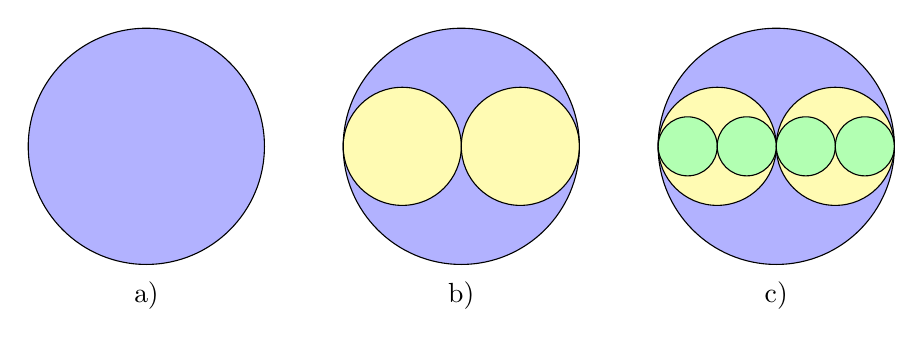
\begin{tikzpicture}
				\begin{scope}
					\fill[blue!30] (0,0) circle (1.5); 
					 \draw (0,0) circle (1.5);
					\node at (0,-1.9) {a)}; 
				\end{scope}
				\begin{scope}[xshift=4cm]
					\fill[blue!30] (0,0)  circle (1.5);
					\foreach \x in  {-0.75,0.75}{
						\fill[yellow!30]  (\x,0) circle (0.75);
						\draw  (\x,0) circle (0.75);
					 }
					\draw  (0,0) circle (1.5);
					\node at (0,-1.9)  {b)};
				\end{scope}
				\begin{scope}[xshift=8cm]
					\fill[blue!30] (0,0) circle (1.5); 
					\foreach \x in {-0.75,0.75}{ 
						\fill[yellow!30] (\x,0) circle  (0.75);
						\draw  (\x,0) circle (0.75);
					} 
					\foreach \x in {-1.125,-0.375,0.375,1.125}{ 
						 \fill[green!30] (\x,0) circle (0.375);
						\draw (\x,0) circle  (0.375);
					 }
					 \draw (0,0) circle (1.5);
					\node at  (0,-1.9) {c)};
				\end{scope}
			\end{tikzpicture}
	\end{center}
	\shortans{628} 
	 \loigiai{
		Gọi $u_1$ là diện  tích của hình tròn đầu tiên, ta có $u_1 = \pi R^2$. \\
		Gọi $u_2$ là tổng diện tích của $2$ hình tròn cắt lần thứ hai, ta có $u_2 = 2 \pi \left( \dfrac{R}{2} \right)^2 = \pi  R^2 \cdot \dfrac{1}{2}$. \\
		Gọi $u_3$ là tổng diện tích của $4$ hình tròn cắt lần thứ ba, ta có $u_3 = 4  \pi \left( \dfrac{R}{4} \right)^2 = \pi R^2 \cdot \dfrac{1}{4}$. \\
		 ...
		Gọi $u_n$ là tổng diện tích của $2^{n-1}$ hình tròn cắt lần thứ $n$, ta có $u_n = 2^{n-1} \pi \left( \dfrac{R}{2^{n-1}} \right)^2 = \pi R^2 \cdot \dfrac{1}{2^{n-1}}$. \\ 
		Dãy $u_1$, $u_2$, $\ldots$, $u_2$, $\ldots$ lập thành một cấp số nhân lùi  vô hạn có $u_1=\pi R^2$ và công bội $q=dfrac{1}{2}$.\\
		 Vậy tổng diện tích của các hình tròn là
		 \[
		S = \pi R^2 + \pi R^2 \cdot \dfrac{1}{2} + \pi R^2 \cdot \dfrac{1}{4} + \ldots = \dfrac{\pi R^2}{1 -  \dfrac{1}{2}} = 2 \pi R^2 = 2 \pi \cdot 10^2 \approx 628.
		 \]
	 }
\end{ex}

% nguồn: Ok_TraLoiNgan_Lop11_Lan2
\begin{ex}%[1D3C1-6]%[ma:f2b5c6db]
	Một bệnh nhân hàng ngày phải uống một viên thuốc $150$\,mg. Sau ngày đầu, trước mỗi lần uống, hàm lượng thuốc cũ trong cơ thể vẫn còn $5\%$. Tính lượng thuốc có trong cơ thể sau khi uống viên  thuốc của ngày thứ $5$. Ước tính lượng thuốc trong cơ thể nếu bệnh nhân sử dụng thuốc trong một thời gian dài.
	 \shortans{1,1}
	\loigiai{ 
		Lượng thuốc trong cơ thể bệnh nhân sau khi uống viên thuốc của ngày đầu  tiên là $150$\,mg. \\
		Sau  ngày đầu, hàm lượng thuốc trong cơ thể sau mỗi ngày là
		\[ 
		S = 150 \left( 1 + 0{,}05 +  0{,}05^2 + 0{,}05^3 + \ldots \right)
		\] 
		Dãy này là tổng  của cấp số nhân lùi vô hạn với số hạng đầu $u_1 = 1$ và công bội $q = 0{,}05$ nên
		\[ 
		S = 150 \cdot \dfrac{1}{1 - 0{,}05} =  \dfrac{400}{361} \approx 1{,}1
		\] 
	 }
\end{ex}

% nguồn: Ok_TraLoiNgan_Lop11_Lan2
\begin{ex}%[1D3C1-6]%[ma:61f2bd7b]
	\immini{ 
	Trong hình vẽ bên, cho đường tròn $(C)$ tâm $O$, bán kính $r = 20$\,cm. Vẽ đường tròn $(C_1)$ đi qua tâm  $O$ và tiếp xúc với $(C)$. Đường tròn $(C_1)$ có bán kính bằng một nửa bán kính của $(C)$, tức là $r_1 = \dfrac{r}{2} = 10$\,cm.
	Tiếp tục, vẽ đường tròn $(C_2)$ đi qua tâm của $(C_1)$ và tiếp xúc với $(C_1)$, với bán kính $r_2 =  \dfrac{r_1}{2} = \dfrac{10}{2} = 5$\,cm.
	Quá trình này tiếp tục đến vô hạn, với mỗi đường tròn mới có bán kính bằng một nửa  bán kính của đường tròn trước đó. Tính diện tích phần tô màu (kết quả làm tròn đến hàng đơn vị).
	} 
	 {
	\begin{tikzpicture}
			\def\a{8} 
			 \def\b{0.5}
			\coordinate (A) at (0,0); 
			\coordinate (B) at  (\a,0);
			 \foreach \i [count=\j from 0] in {2,4,8}{
				\coordinate (O\j)  at ($(A)!\b^(1+\j)!(B)$);
				 \fill[gray!\i0] (O\j) circle (\a/\i);
				\draw (O\j) circle (\a/\i); 
				 \draw (\a/\i,-\a/\i) -- (\a/\i,\a/\i);
				\fill[white] (\a/\i,-\a/\i) arc[start angle=-90,end angle=90,radius=\a/\i];
			} 
			\fill[white]  (\a/16,0) circle (\a/16);
			 \fill[white] (\a/16,0) circle (\a/16);
			\draw[dashed]  (A)--(B);
			\foreach \j/\label in {0/O,1/O_1,2/O_2}{ 
				\fill (O\j) circle (1pt)  node[xshift=6pt,yshift=-6pt] {$\label$};
			 }
			\fill  (A) circle (1pt) node[xshift=-6pt,yshift=-6pt] {$A$};
			\fill (\a/16,0) circle  (1pt) node[xshift=3pt,yshift=-6pt] {$O_3$};
		\end{tikzpicture}
	 }
	\shortans{419} 
	 \loigiai{
		Diện tích của đường tròn ban đầu $(C)$ là $S_0  = \pi r^2 = \pi \cdot 20^2 = 400\pi$\,cm$^2$.\\
		Diện tích của $(C_1)$ là $S_1 = \pi r_1^2 = \pi \cdot 10^2  = 100\pi$\,cm$^2$.\\
		Diện tích của $(C_2)$ là $S_2 = \pi r_2^2 = \pi  \cdot 5^2 = 25\pi$\,cm$^2$.\\
		Tiếp tục như vậy, diện tích của các đường tròn tạo thành một cấp  số nhân với số hạng đầu $S_1 = 100\pi$ và công bội $q = \dfrac{1}{4}$.\\
		Phần tô màu là  tổng diện tích của các đường tròn $(C_1), (C_2), (C_3), \dots$ ngoại trừ diện tích của $(C)$. \\
		Tổng diện tích phần tô  màu là tổng của một cấp số nhân lùi vô hạn
		 \[
		S = S_1 + S_2 + S_3 + \dots = \dfrac{S_1}{1  - q} = \dfrac{100\pi}{1 - \dfrac{1}{4}} = \dfrac{100\pi}{\dfrac{3}{4}} = \dfrac{400\pi}{3}.
		 \]
		Vậy, diện tích  toàn bộ phần tô màu là
		 \[
		S = \dfrac{400\pi}{3} \approx 419 \text{  cm}^2.
		 \]
	 }
\end{ex}

% nguồn: Ok_TraLoiNgan_Lop11_Lan2
\begin{ex}%[1D3C1-6]%[ma:0fe44c43]
	Xét quá trình tạo ra hình có chu vi vô  cực và diện tích bằng $0$ như sau: \\
	Bắt đầu bằng một hình vuông $H_0$ cạnh bằng $1$ đơn vị độ dài. Chia hình vuông $H_0$ thành chín hình vuông bằng nhau, bỏ đi bốn hình vuông, nhận được hình  $H_1$. Tiếp tục quá trình này với mỗi hình vuông của $H_1$, chia thành chín phần rồi bỏ đi bốn hình vuông, nhận được hình $H_2$. Quá trình này tiếp diễn vô hạn ta nhận được một dãy hình $H_n\,(n=1,2,3,...)$. Gọi $S_n$ là diện tích của $H_n$. Tính $\lim S_n$.
	\begin{center}
		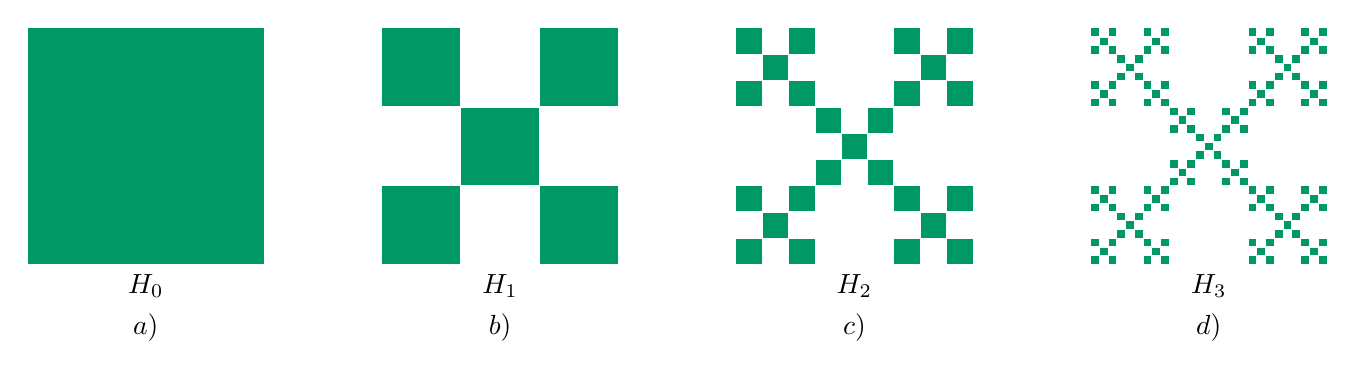
\begin{tikzpicture}
				 \def\a{1.5}
				 \pgfmathsetmacro\sh{2*\a *sqrt (2)/3}
				\def\hv#1{ 
				 \ifnum#1>0
				 \draw[white,fill=white]
					(-\a/3,\a/3) rectangle  (\a/3,\a)
					 (-\a/3,-\a/3) rectangle (-\a,\a/3)
					 (-\a/3,-\a/3) rectangle (\a/3,-\a)
					(\a/3,-\a/3) rectangle (\a,\a/3); 
				\pgfmathtruncatemacro{\k}{#1-1} 
			\begin{scope}[scale=1/3]\hv{\k}\end{scope}
			\begin{scope}[shift={(45:\sh)},scale=1/3]\hv{\k}\end{scope}
			\begin{scope}[shift={(135:\sh)},scale=1/3]\hv{\k}\end{scope}
			\begin{scope}[shift={(225:\sh)},scale=1/3]\hv{\k}\end{scope}
			\begin{scope}[shift={(315:\sh)},scale=1/3]\hv{\k}\end{scope}
				\fi 
				} 
				\begin{scope}
					\fill[blue!40!green] (-\a,-\a)  rectangle (\a,\a);
					 \hv{0}
					 \path (0,-\a) node[below]{$H_0$}
						 node[below=.5cm]{$a)$};
				\end{scope}
				\begin{scope}[xshift=4.5cm]
					\fill[blue!40!green] (-\a,-\a) rectangle (\a,\a); 
					 \hv{1}
					\path (0,-\a) node[below]{$H_1$} 
						 node[below=.5cm]{$b)$};
				\end{scope}
				\begin{scope}[xshift=9cm]
					\fill[blue!40!green]  (-\a,-\a) rectangle (\a,\a);
					 \hv{2}
					\path  (0,-\a) node[below]{$H_2$}
						 node[below=.5cm]{$c)$};
				\end{scope}
				\begin{scope}[xshift=13.5cm]
					\fill[blue!40!green] (-\a,-\a) rectangle (\a,\a); 
					 \hv{3}
					\path (0,-\a)  node[below]{$H_3$}
						node[below=.5cm]{$d)$}; 
				\end{scope}
			\end{tikzpicture}
	\end{center}
	\shortans{0} 
	 \loigiai{
		Ta có $H_1$ có $5$ hình vuông, mỗi hình vuông  có cạnh bằng $\dfrac{1}{3}$; \\
		$H_2$ có $5 \cdot 5 = 5^2$ hình vuông, mỗi hình vuông có cạnh bằng $\dfrac{1}{3} \cdot  \dfrac{1}{3} = \dfrac{1}{3^2}$. \\
		Tương  tự, $H_n$ sẽ có $5^n$ hình vuông, mỗi hình vuông có cạnh bằng $\dfrac{1}{3^n}$.\\
		Diện tích $S_n$ của  $H_n$ là
		\[ 
		S_n = 5^n \cdot \left( \dfrac{1}{3} \right)^n \cdot \left( \dfrac{1}{3} \right)^n =  5^n \cdot \left( \dfrac{1}{3} \right)^{2n} = \left( \dfrac{5}{9} \right)^n
		\] 
		Vì  $\dfrac{5}{9} < 1$, nên $\lim S_n = \lim \left( \dfrac{5}{9} \right)^n = 0$.
	} 
\end{ex}
